% Chapter 6

\chapter[Video Tracking System]{Video Tracking System} % Main chapter title

\label{Chapter6} % For referencing the chapter elsewhere, use \ref{Chapter6} 

%----------------------------------------------------------------------------------------

In order to implement the augmented reality element of the system, and satisfy the related objectives, a live video feed of the swarm was needed. A method for tracking the positions of each individual robot in the swarm within each video frame in this feed was also required, in order to correctly position the graphical overlays. Prior to the start of this project infrastructure had been put in place at the YRL for performing this kind of video-based tracking task, in the form of a machine vision camera placed above an 'arena'. Figure \ref{fig:CameraLayout} shows the arrangement of the machine vision camera used for robot tracking, and the robot arena. Figure \ref{fig:ArenaPhoto} shows a photo of the robot arena and tracking camera set up at the YRL. Ongoing research being carried out by members of the YRL had already made use of this camera and arena set up, in conjunction with image processing software for tracking fiducial markers within the image, to achieve robot tracking with good accuracy and relatively high frame-rate.

\begin{figure}[h]
	\centering
	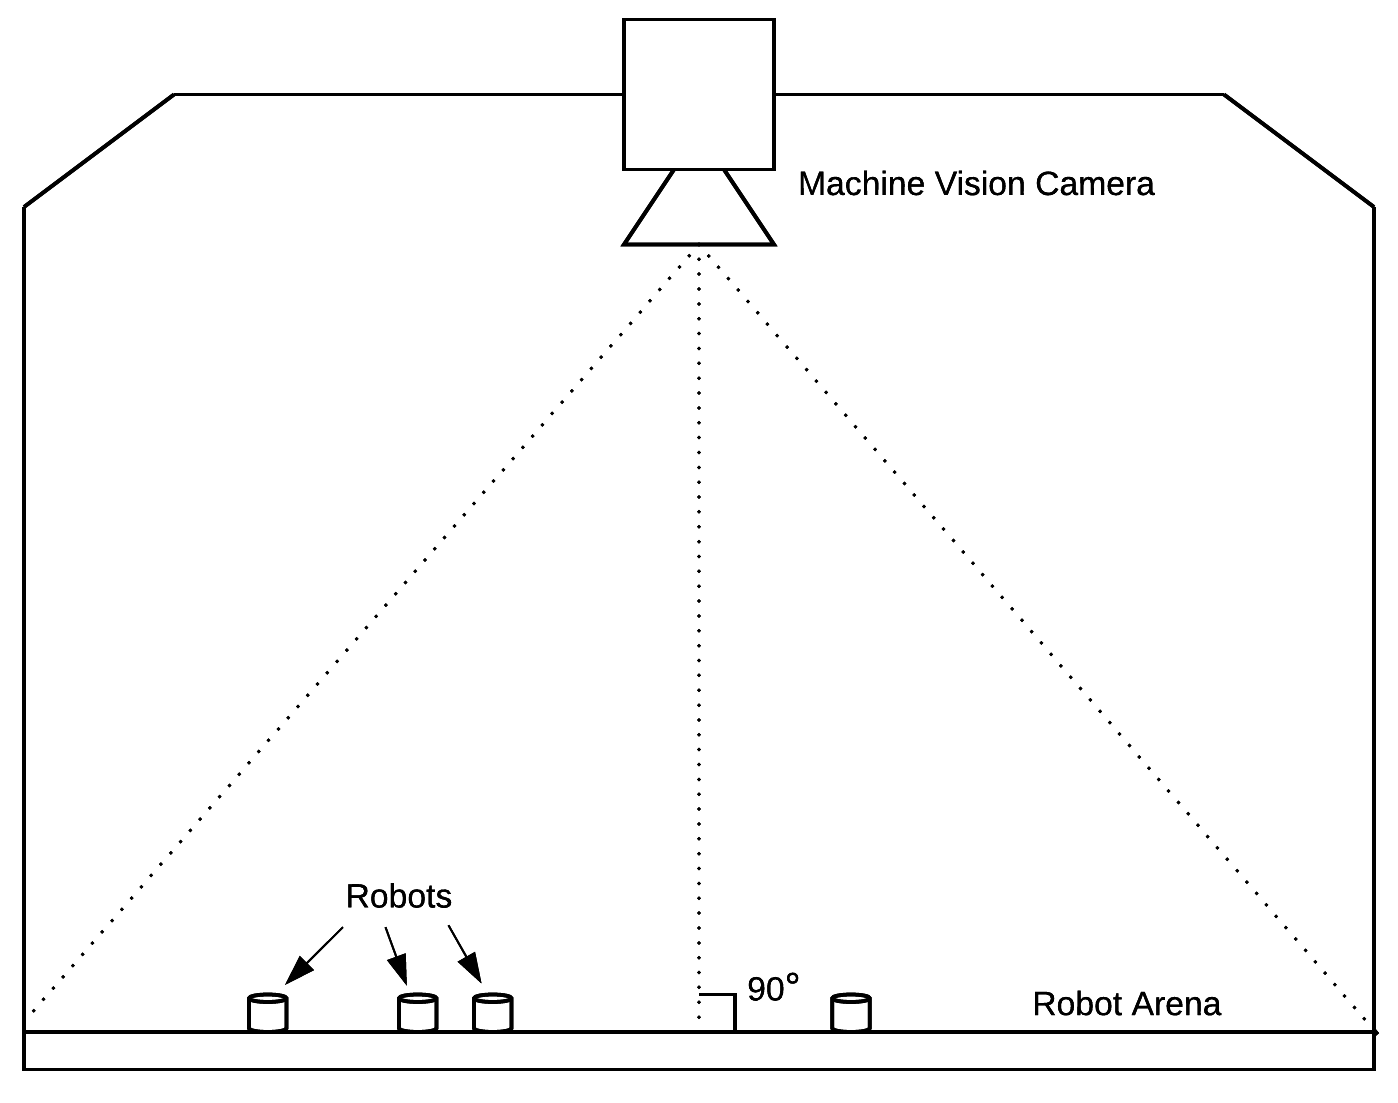
\includegraphics[scale=0.3]{Figures/CameraLayout.png}
	\decoRule
	\caption[Tracking Camera Arrangement]{Arrangement of the tracking camera over the robot arena.}
	\label{fig:CameraLayout}
\end{figure}

The image processing in these ongoing research efforts was performed using the `ARuCo\cite{Garrido:2014}' fiducial marker based tracking system, discussed further in section \ref{ARuCo}. It was determined that incorporating this existing infrastructure into this project would be the quickest way to achieve an operational tracking system, allowing work to focus on the novel aspects of this project sooner.

\begin{figure}
	\centering
	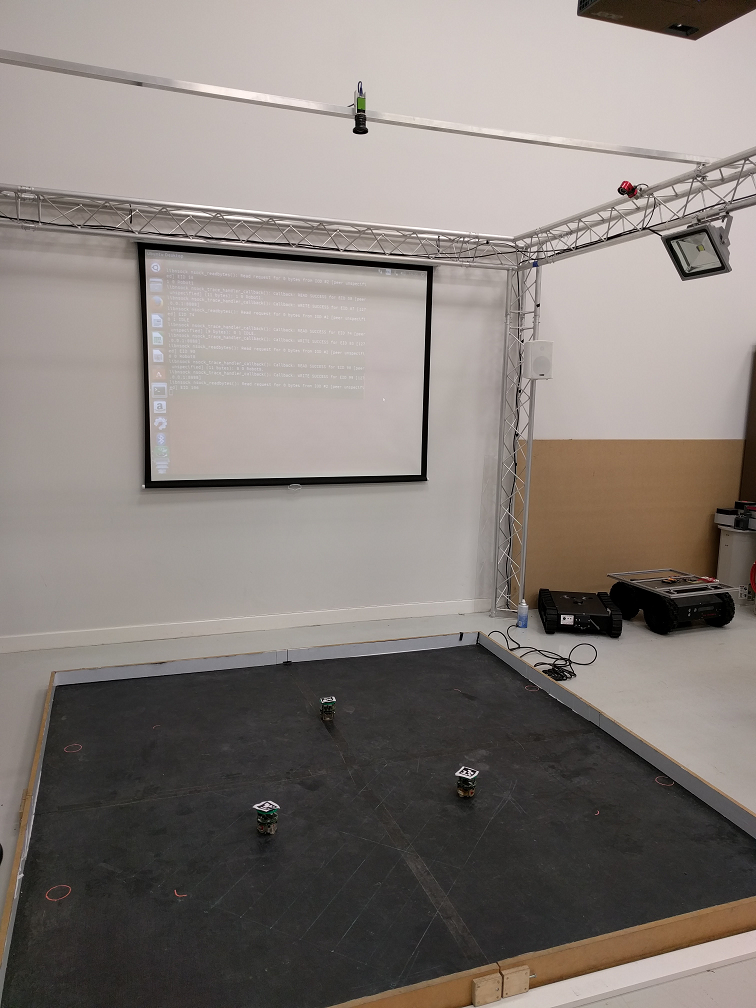
\includegraphics[scale=0.4]{Figures/ArenaPhoto.png}
	\decoRule
	\caption[Robot Arena and Tracking Camera]{The robot arena set up at the YRL, with tracking camera visible.}
	\label{fig:ArenaPhoto}
\end{figure}

%----------------------------------------------------------------------------------------

\section{Camera}
The camera used in the aforementioned tracking set-up is a JAI Go 5000C-PGE colour, area-scan camera. It features a 1-inch, 5-megapixel CMOS sensor, with a maximum resolution of 2560 by 2048 pixels, capable of capturing 22 frames per second at full resolution, and up to 163.5 frames per second with reduced resolution and colour quality. The camera also features a global shutter, meaning it captures the full area of the image simultaneously, as opposed to a rolling shutter 


%----------------------------------------------------------------------------------------

\section{ARuCo Tracking System} \label{ARuCo}
Developed by a team from the Computing and Numerical Analysis Department at Cordoba University in Spain, the ARuCo tag generation and detection system \cite{Garrido:2014} is a powerful fiducial marker creation and tracking tool. It comprises an algorithm for producing a `dictionary' of square, black and white, coded markers which can be printed and attached to objects and surfaces, and a method for automatically detecting these markers in a given image. The stated applications include augmented reality and robot localisation. One of the main benefits of this system over other fiducial marker systems is the execution speed. By first using edge-detection methods to find the outlines of markers in the image, the system can eliminate a large portion of the image before applying the more complex processing to identify and differentiate individual tags \cite{Garrido:2014}. This makes it possible for the ARuCo system to be run in real time, even with relatively modest computational power. In a conventional use case the orientation of the camera can be calculated based on the positions of the corners of a tag, given that the tag's orientation is known. In this use case the reverse is true, the camera's position is fixed, and therefore the orientation of the robot can be determined based on the position and orientation of the corners of its tag, relative to the camera. 

Each of the e-puck robots used in this project were assigned an ID number, and a dictionary of ARuCo tags was generated to match. The tags were affixed to the top of the robots, oriented to match their forward directions. Some cursory preliminary testing showed that the tags could be accurately and reliably detected in the camera images, at a decent frame rate. Further detail of the integration of the ARuCo marker tracking system into this application is given in section \ref{VideoFeedAndTrackingSystem}.

%----------------------------------------------------------------------------------------